\chapter {チャプター名}
\label{chap:提案手法}
本論文で行う実験は,数値計算を固定小数点によって計算することである.
浮動小数点を用いて計算することの多い問題に対して固定小数点を用いて計算する方が計算結果の精度が高くなる場合があると考える.
次の章では,数値実験によって等しいbit数の固定小数点と浮動小数点を用いて実験を行った.


第\ref{chap:基礎知識1}章で述べたように,固定小数点と浮動小数点では表現できる数のうち隣り合う2数の間隔が異なる範囲がある.
そのため,固定小数点と浮動小数点では計算の過程で扱う数の範囲によって計算機の中で表現できる数の個数が異なる. %この文変だなぁ。
本論文では,ある数値型$\mathrm{T}$と計算機で扱う数の範囲$I \subset \R$を用いて,範囲$I$での数値型$\mathrm{T}$の密度${|I|}_{\mathrm{T}}$を以下のように定義する.
\begin{align}
    \label{eq:def_density}
    {|I|}_{\mathrm{T}}: \text{集合}\left\{x^{\ast} \ | \ x^{\ast} \in \mathbb{F}_{\mathrm{T}} \cap I \right\}\text{の要素の数.}
\end{align}
ただし,数値型$\mathrm{T}$で表せる最大の数を$M_{\mathrm{T}}$,最小の数を$m_{\mathrm{T}}$とし,
\begin{equation}
    I \subset (m_{\mathrm{T}}, M_{\mathrm{T}})
\end{equation}
とする.
例として,8bitの固定小数点(Q4f3)を考える.
このとき,
\begin{align}
    m_{\mathrm{Q}4\mathrm{f}3} &= -14.875, \\
    M_{\mathrm{Q}4\mathrm{f}3} &= 14.875
\end{align}
であり,$I$を
\begin{eqnarray}
    I = \left(-3,2\right)
\end{eqnarray}
とすると,${|\left(-3,2\right)|}_{\mathrm{Q}4\mathrm{f}3}$は,
\begin{align}
    &\left\{x^{\ast}\in \fixnumcustom{4}{3} \cap (-3,2)\right\} \\
    &= \left\{-2.875,-2.750,-2.625,\dots,1.625,1.750,1.875\right\}
\end{align}
となるため,
\begin{align}
    {|I|}_{\mathrm{Q}4\mathrm{f}3} = 39
\end{align}
となる.
このように定義した密度${|I|}_{\mathrm{T}}$を用いて,同じ範囲$J \in \R$に対して異なる数値型$T_1,T_2$で計算を行うことを考える.
ただし,
\begin{equation}
    J \subset (m_{T_1}, M_{T_1}) \cap (m_{T_2}, M_{T_2})
\end{equation}
とする.
また,
\begin{equation}
    {|J|}_{T_1} < {|J|}_{T_2}
\end{equation}
と仮定する.

\begin{figure}[H]
    \centering
    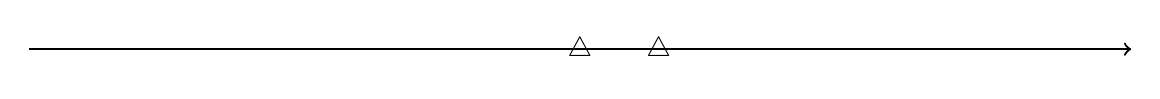
\begin{tikzpicture}
        \node (A) at (0,0) {$\bigtriangleup$};
        \draw [->, thick] (-7,0) -- (7,0);
        \node (B) at (1,0) {$\bigtriangleup$};
    \end{tikzpicture}
\end{figure}

